\documentclass[twoside]{book}

% Packages required by doxygen
\usepackage{fixltx2e}
\usepackage{calc}
\usepackage{doxygen}
\usepackage[export]{adjustbox} % also loads graphicx
\usepackage{graphicx}
\usepackage[utf8]{inputenc}
\usepackage{makeidx}
\usepackage{multicol}
\usepackage{multirow}
\PassOptionsToPackage{warn}{textcomp}
\usepackage{textcomp}
\usepackage[nointegrals]{wasysym}
\usepackage[table]{xcolor}

% Font selection
\usepackage[T1]{fontenc}
\usepackage[scaled=.90]{helvet}
\usepackage{courier}
\usepackage{amssymb}
\usepackage{sectsty}
\renewcommand{\familydefault}{\sfdefault}
\allsectionsfont{%
  \fontseries{bc}\selectfont%
  \color{darkgray}%
}
\renewcommand{\DoxyLabelFont}{%
  \fontseries{bc}\selectfont%
  \color{darkgray}%
}
\newcommand{\+}{\discretionary{\mbox{\scriptsize$\hookleftarrow$}}{}{}}

% Page & text layout
\usepackage{geometry}
\geometry{%
  a4paper,%
  top=2.5cm,%
  bottom=2.5cm,%
  left=2.5cm,%
  right=2.5cm%
}
\tolerance=750
\hfuzz=15pt
\hbadness=750
\setlength{\emergencystretch}{15pt}
\setlength{\parindent}{0cm}
\setlength{\parskip}{3ex plus 2ex minus 2ex}
\makeatletter
\renewcommand{\paragraph}{%
  \@startsection{paragraph}{4}{0ex}{-1.0ex}{1.0ex}{%
    \normalfont\normalsize\bfseries\SS@parafont%
  }%
}
\renewcommand{\subparagraph}{%
  \@startsection{subparagraph}{5}{0ex}{-1.0ex}{1.0ex}{%
    \normalfont\normalsize\bfseries\SS@subparafont%
  }%
}
\makeatother

% Headers & footers
\usepackage{fancyhdr}
\pagestyle{fancyplain}
\fancyhead[LE]{\fancyplain{}{\bfseries\thepage}}
\fancyhead[CE]{\fancyplain{}{}}
\fancyhead[RE]{\fancyplain{}{\bfseries\leftmark}}
\fancyhead[LO]{\fancyplain{}{\bfseries\rightmark}}
\fancyhead[CO]{\fancyplain{}{}}
\fancyhead[RO]{\fancyplain{}{\bfseries\thepage}}
\fancyfoot[LE]{\fancyplain{}{}}
\fancyfoot[CE]{\fancyplain{}{}}
\fancyfoot[RE]{\fancyplain{}{\bfseries\scriptsize Generated by Doxygen }}
\fancyfoot[LO]{\fancyplain{}{\bfseries\scriptsize Generated by Doxygen }}
\fancyfoot[CO]{\fancyplain{}{}}
\fancyfoot[RO]{\fancyplain{}{}}
\renewcommand{\footrulewidth}{0.4pt}
\renewcommand{\chaptermark}[1]{%
  \markboth{#1}{}%
}
\renewcommand{\sectionmark}[1]{%
  \markright{\thesection\ #1}%
}

% Indices & bibliography
\usepackage{natbib}
\usepackage[titles]{tocloft}
\setcounter{tocdepth}{3}
\setcounter{secnumdepth}{5}
\makeindex

% Hyperlinks (required, but should be loaded last)
\usepackage{ifpdf}
\ifpdf
  \usepackage[pdftex,pagebackref=true]{hyperref}
\else
  \usepackage[ps2pdf,pagebackref=true]{hyperref}
\fi
\hypersetup{%
  colorlinks=true,%
  linkcolor=blue,%
  citecolor=blue,%
  unicode%
}

% Custom commands
\newcommand{\clearemptydoublepage}{%
  \newpage{\pagestyle{empty}\cleardoublepage}%
}

\usepackage{caption}
\captionsetup{labelsep=space,justification=centering,font={bf},singlelinecheck=off,skip=4pt,position=top}

%===== C O N T E N T S =====

\begin{document}

% Titlepage & ToC
\hypersetup{pageanchor=false,
             bookmarksnumbered=true,
             pdfencoding=unicode
            }
\pagenumbering{alph}
\begin{titlepage}
\vspace*{7cm}
\begin{center}%
{\Large R\+OS Control }\\
\vspace*{1cm}
{\large Generated by Doxygen 1.8.13}\\
\end{center}
\end{titlepage}
\clearemptydoublepage
\pagenumbering{roman}
\tableofcontents
\clearemptydoublepage
\pagenumbering{arabic}
\hypersetup{pageanchor=true}

%--- Begin generated contents ---
\chapter{R\+OS Control x Jetracer}
\label{md__r_e_a_d_m_e}
\Hypertarget{md__r_e_a_d_m_e}
\input{md__r_e_a_d_m_e}
\chapter{Hierarchical Index}
\section{Class Hierarchy}
This inheritance list is sorted roughly, but not completely, alphabetically\+:\begin{DoxyCompactList}
\item Generic\+H\+W\+Interface\begin{DoxyCompactList}
\item \contentsline{section}{fennec\+\_\+ns\+:\+:Fennec\+H\+W\+Interface}{\pageref{classfennec__ns_1_1_fennec_h_w_interface}}{}
\end{DoxyCompactList}
\item \contentsline{section}{I2\+C\+\_\+\+Driver}{\pageref{class_i2_c___driver}}{}
\item \contentsline{section}{P\+C\+A9685}{\pageref{class_p_c_a9685}}{}
\end{DoxyCompactList}

\chapter{Class Index}
\section{Class List}
Here are the classes, structs, unions and interfaces with brief descriptions\+:\begin{DoxyCompactList}
\item\contentsline{section}{\hyperlink{classfennec__ns_1_1_fennec_h_w_interface}{fennec\+\_\+ns\+::\+Fennec\+H\+W\+Interface} \\*Hardware interface for a robot }{\pageref{classfennec__ns_1_1_fennec_h_w_interface}}{}
\item\contentsline{section}{\hyperlink{class_i2_c___driver}{I2\+C\+\_\+\+Driver} }{\pageref{class_i2_c___driver}}{}
\item\contentsline{section}{\hyperlink{class_p_c_a9685}{P\+C\+A9685} }{\pageref{class_p_c_a9685}}{}
\end{DoxyCompactList}

\chapter{Class Documentation}
\hypertarget{classfennec__ns_1_1_fennec_h_w_interface}{}\section{fennec\+\_\+ns\+:\+:Fennec\+H\+W\+Interface Class Reference}
\label{classfennec__ns_1_1_fennec_h_w_interface}\index{fennec\+\_\+ns\+::\+Fennec\+H\+W\+Interface@{fennec\+\_\+ns\+::\+Fennec\+H\+W\+Interface}}


Hardware interface for a robot.  




{\ttfamily \#include $<$fennec\+\_\+hw\+\_\+interface.\+h$>$}



Inheritance diagram for fennec\+\_\+ns\+:\+:Fennec\+H\+W\+Interface\+:
\nopagebreak
\begin{figure}[H]
\begin{center}
\leavevmode
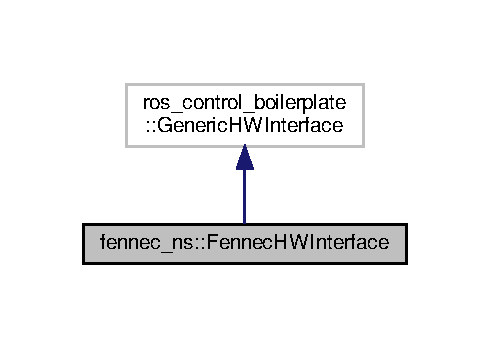
\includegraphics[width=235pt]{classfennec__ns_1_1_fennec_h_w_interface__inherit__graph}
\end{center}
\end{figure}


Collaboration diagram for fennec\+\_\+ns\+:\+:Fennec\+H\+W\+Interface\+:
\nopagebreak
\begin{figure}[H]
\begin{center}
\leavevmode
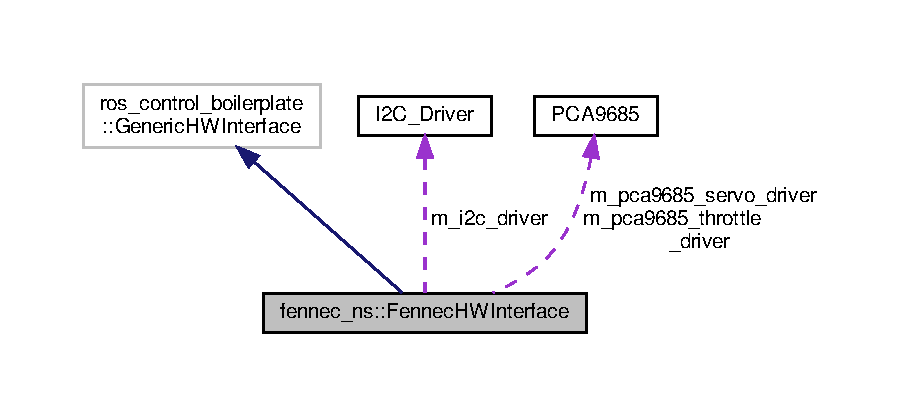
\includegraphics[width=350pt]{classfennec__ns_1_1_fennec_h_w_interface__coll__graph}
\end{center}
\end{figure}
\subsection*{Public Member Functions}
\begin{DoxyCompactItemize}
\item 
\hyperlink{classfennec__ns_1_1_fennec_h_w_interface_a2efa0dd31094aa112588ba5ca1ff6f69}{Fennec\+H\+W\+Interface} (ros\+::\+Node\+Handle \&nh, urdf\+::\+Model $\ast$urdf\+\_\+model=N\+U\+LL)
\begin{DoxyCompactList}\small\item\em Constructor. \end{DoxyCompactList}\item 
\mbox{\Hypertarget{classfennec__ns_1_1_fennec_h_w_interface_a26858f1a85875199f276e12d5fe30113}\label{classfennec__ns_1_1_fennec_h_w_interface_a26858f1a85875199f276e12d5fe30113}} 
virtual \hyperlink{classfennec__ns_1_1_fennec_h_w_interface_a26858f1a85875199f276e12d5fe30113}{$\sim$\+Fennec\+H\+W\+Interface} ()
\begin{DoxyCompactList}\small\item\em Destroy the Fennec HW Interface\+:\+: Fennec HW Interface object. \end{DoxyCompactList}\item 
virtual void \hyperlink{classfennec__ns_1_1_fennec_h_w_interface_ad5e55d24cc4471e666f2e5e17977ca13}{init} ()
\begin{DoxyCompactList}\small\item\em Initialize the robot hardware interface. \end{DoxyCompactList}\item 
virtual void \hyperlink{classfennec__ns_1_1_fennec_h_w_interface_adb8bbfce4a97c7f0a007a6ddf933be7a}{read} (ros\+::\+Duration \&elapsed\+\_\+time)
\begin{DoxyCompactList}\small\item\em Read the state from the robot hardware. \end{DoxyCompactList}\item 
virtual void \hyperlink{classfennec__ns_1_1_fennec_h_w_interface_a0b68acf47d161d3c7d30d21b35327923}{write} (ros\+::\+Duration \&elapsed\+\_\+time)
\begin{DoxyCompactList}\small\item\em Write the command to the robot hardware. \end{DoxyCompactList}\item 
virtual void \hyperlink{classfennec__ns_1_1_fennec_h_w_interface_a30250e644ed2ef16ee724289c8193066}{enforce\+Limits} (ros\+::\+Duration \&period)
\item 
void \hyperlink{classfennec__ns_1_1_fennec_h_w_interface_a918620ccc3c2bc7852b2f9e5fa90c54c}{encoder\+Callback} (const std\+\_\+msgs\+::\+Int16\+::\+Const\+Ptr \&msg)
\begin{DoxyCompactList}\small\item\em Counts the pulses of the encoder. Gets called everytime the rosserial node publishes a new msg. \end{DoxyCompactList}\item 
\mbox{\Hypertarget{classfennec__ns_1_1_fennec_h_w_interface_ae3d579b889bed76ab21335d767ac4ed4}\label{classfennec__ns_1_1_fennec_h_w_interface_ae3d579b889bed76ab21335d767ac4ed4}} 
void \hyperlink{classfennec__ns_1_1_fennec_h_w_interface_ae3d579b889bed76ab21335d767ac4ed4}{print\+Commands} ()
\begin{DoxyCompactList}\small\item\em A helper function to print the R\+OS Controller Commands for each control loop to the console. \end{DoxyCompactList}\end{DoxyCompactItemize}
\subsection*{Public Attributes}
\begin{DoxyCompactItemize}
\item 
\mbox{\Hypertarget{classfennec__ns_1_1_fennec_h_w_interface_a9e450fc1f1b96701f89be637a58622a9}\label{classfennec__ns_1_1_fennec_h_w_interface_a9e450fc1f1b96701f89be637a58622a9}} 
const char $\ast$ \hyperlink{classfennec__ns_1_1_fennec_h_w_interface_a9e450fc1f1b96701f89be637a58622a9}{m\+\_\+i2c\+\_\+device\+\_\+name} = \char`\"{}/dev/i2c-\/1\char`\"{}
\begin{DoxyCompactList}\small\item\em The I2C Bus 1 is used by the \hyperlink{class_p_c_a9685}{P\+C\+A9685} boards. \end{DoxyCompactList}\item 
\mbox{\Hypertarget{classfennec__ns_1_1_fennec_h_w_interface_a62c8cef371f076986ead0942304d134c}\label{classfennec__ns_1_1_fennec_h_w_interface_a62c8cef371f076986ead0942304d134c}} 
\hyperlink{class_i2_c___driver}{I2\+C\+\_\+\+Driver} $\ast$ {\bfseries m\+\_\+i2c\+\_\+driver} = new \hyperlink{class_i2_c___driver}{I2\+C\+\_\+\+Driver}(\hyperlink{classfennec__ns_1_1_fennec_h_w_interface_a9e450fc1f1b96701f89be637a58622a9}{m\+\_\+i2c\+\_\+device\+\_\+name})
\item 
\mbox{\Hypertarget{classfennec__ns_1_1_fennec_h_w_interface_aad562b8627b08e5dfdda168ade82530d}\label{classfennec__ns_1_1_fennec_h_w_interface_aad562b8627b08e5dfdda168ade82530d}} 
const uint8\+\_\+t \hyperlink{classfennec__ns_1_1_fennec_h_w_interface_aad562b8627b08e5dfdda168ade82530d}{m\+\_\+steering\+\_\+pca9685\+\_\+address} = 0x40
\begin{DoxyCompactList}\small\item\em The default adress for a \hyperlink{class_p_c_a9685}{P\+C\+A9685} board. \end{DoxyCompactList}\item 
\mbox{\Hypertarget{classfennec__ns_1_1_fennec_h_w_interface_af8ebee84c63d1be3c949d58ab6087dbc}\label{classfennec__ns_1_1_fennec_h_w_interface_af8ebee84c63d1be3c949d58ab6087dbc}} 
\hyperlink{class_p_c_a9685}{P\+C\+A9685} $\ast$ {\bfseries m\+\_\+pca9685\+\_\+servo\+\_\+driver} = new \hyperlink{class_p_c_a9685}{P\+C\+A9685}(m\+\_\+i2c\+\_\+driver, \hyperlink{classfennec__ns_1_1_fennec_h_w_interface_aad562b8627b08e5dfdda168ade82530d}{m\+\_\+steering\+\_\+pca9685\+\_\+address})
\item 
\mbox{\Hypertarget{classfennec__ns_1_1_fennec_h_w_interface_a515996ba43ee57670c6275b560997876}\label{classfennec__ns_1_1_fennec_h_w_interface_a515996ba43ee57670c6275b560997876}} 
const uint8\+\_\+t \hyperlink{classfennec__ns_1_1_fennec_h_w_interface_a515996ba43ee57670c6275b560997876}{m\+\_\+throttle\+\_\+pca9685\+\_\+address} = 0x60
\begin{DoxyCompactList}\small\item\em The adress of the 2nd \hyperlink{class_p_c_a9685}{P\+C\+A9685} board. \end{DoxyCompactList}\item 
\mbox{\Hypertarget{classfennec__ns_1_1_fennec_h_w_interface_a6a6def1f04ecb0ca88b659aca69cfa60}\label{classfennec__ns_1_1_fennec_h_w_interface_a6a6def1f04ecb0ca88b659aca69cfa60}} 
\hyperlink{class_p_c_a9685}{P\+C\+A9685} $\ast$ {\bfseries m\+\_\+pca9685\+\_\+throttle\+\_\+driver} = new \hyperlink{class_p_c_a9685}{P\+C\+A9685}(m\+\_\+i2c\+\_\+driver, \hyperlink{classfennec__ns_1_1_fennec_h_w_interface_a515996ba43ee57670c6275b560997876}{m\+\_\+throttle\+\_\+pca9685\+\_\+address})
\item 
\mbox{\Hypertarget{classfennec__ns_1_1_fennec_h_w_interface_ab1ca5a0a877c3bd02fcc2c93c8b85e60}\label{classfennec__ns_1_1_fennec_h_w_interface_ab1ca5a0a877c3bd02fcc2c93c8b85e60}} 
int16\+\_\+t \hyperlink{classfennec__ns_1_1_fennec_h_w_interface_ab1ca5a0a877c3bd02fcc2c93c8b85e60}{m\+\_\+old\+\_\+num\+\_\+pulses}
\begin{DoxyCompactList}\small\item\em Needed for calculating the driven rear wheel distance. \end{DoxyCompactList}\item 
\mbox{\Hypertarget{classfennec__ns_1_1_fennec_h_w_interface_a117444fd6f01a83c603bc3ff6b7a3ffe}\label{classfennec__ns_1_1_fennec_h_w_interface_a117444fd6f01a83c603bc3ff6b7a3ffe}} 
int \hyperlink{classfennec__ns_1_1_fennec_h_w_interface_a117444fd6f01a83c603bc3ff6b7a3ffe}{m\+\_\+difference\+\_\+num\+\_\+of\+\_\+pulses}
\begin{DoxyCompactList}\small\item\em Needed for calculating the driven rear wheel distance. \end{DoxyCompactList}\item 
\mbox{\Hypertarget{classfennec__ns_1_1_fennec_h_w_interface_a2ff004471cd398edf8ab25e0e34d8f2e}\label{classfennec__ns_1_1_fennec_h_w_interface_a2ff004471cd398edf8ab25e0e34d8f2e}} 
int \hyperlink{classfennec__ns_1_1_fennec_h_w_interface_a2ff004471cd398edf8ab25e0e34d8f2e}{m\+\_\+difference\+\_\+num\+\_\+pulses\+\_\+since\+\_\+last\+\_\+read}
\begin{DoxyCompactList}\small\item\em Needed for calculating the driven rear wheel distance. \end{DoxyCompactList}\item 
\mbox{\Hypertarget{classfennec__ns_1_1_fennec_h_w_interface_af8946e6a059010374d152c428e75c252}\label{classfennec__ns_1_1_fennec_h_w_interface_af8946e6a059010374d152c428e75c252}} 
const u\+\_\+int8\+\_\+t {\bfseries servo\+\_\+channel} = 0
\item 
\mbox{\Hypertarget{classfennec__ns_1_1_fennec_h_w_interface_a57306686ca8d401e8ee6c71c77c2b47c}\label{classfennec__ns_1_1_fennec_h_w_interface_a57306686ca8d401e8ee6c71c77c2b47c}} 
ros\+::\+Subscriber \hyperlink{classfennec__ns_1_1_fennec_h_w_interface_a57306686ca8d401e8ee6c71c77c2b47c}{rosserial\+\_\+sub}
\begin{DoxyCompactList}\small\item\em Subscriber to the /encoder\+\_\+pulses topic, which is published by the Arduino. \end{DoxyCompactList}\item 
\mbox{\Hypertarget{classfennec__ns_1_1_fennec_h_w_interface_afdb8c91b694144d8f4cd05780e15b0c1}\label{classfennec__ns_1_1_fennec_h_w_interface_afdb8c91b694144d8f4cd05780e15b0c1}} 
bool \hyperlink{classfennec__ns_1_1_fennec_h_w_interface_afdb8c91b694144d8f4cd05780e15b0c1}{logging}
\begin{DoxyCompactList}\small\item\em Can be changed at runtime with a R\+OS Param. \end{DoxyCompactList}\end{DoxyCompactItemize}


\subsection{Detailed Description}
Hardware interface for a robot. 

\subsection{Constructor \& Destructor Documentation}
\mbox{\Hypertarget{classfennec__ns_1_1_fennec_h_w_interface_a2efa0dd31094aa112588ba5ca1ff6f69}\label{classfennec__ns_1_1_fennec_h_w_interface_a2efa0dd31094aa112588ba5ca1ff6f69}} 
\index{fennec\+\_\+ns\+::\+Fennec\+H\+W\+Interface@{fennec\+\_\+ns\+::\+Fennec\+H\+W\+Interface}!Fennec\+H\+W\+Interface@{Fennec\+H\+W\+Interface}}
\index{Fennec\+H\+W\+Interface@{Fennec\+H\+W\+Interface}!fennec\+\_\+ns\+::\+Fennec\+H\+W\+Interface@{fennec\+\_\+ns\+::\+Fennec\+H\+W\+Interface}}
\subsubsection{\texorpdfstring{Fennec\+H\+W\+Interface()}{FennecHWInterface()}}
{\footnotesize\ttfamily fennec\+\_\+ns\+::\+Fennec\+H\+W\+Interface\+::\+Fennec\+H\+W\+Interface (\begin{DoxyParamCaption}\item[{ros\+::\+Node\+Handle \&}]{nh,  }\item[{urdf\+::\+Model $\ast$}]{urdf\+\_\+model = {\ttfamily NULL} }\end{DoxyParamCaption})}



Constructor. 


\begin{DoxyParams}{Parameters}
{\em nh} & -\/ Node handle for topics. \\
\hline
\end{DoxyParams}


\subsection{Member Function Documentation}
\mbox{\Hypertarget{classfennec__ns_1_1_fennec_h_w_interface_a918620ccc3c2bc7852b2f9e5fa90c54c}\label{classfennec__ns_1_1_fennec_h_w_interface_a918620ccc3c2bc7852b2f9e5fa90c54c}} 
\index{fennec\+\_\+ns\+::\+Fennec\+H\+W\+Interface@{fennec\+\_\+ns\+::\+Fennec\+H\+W\+Interface}!encoder\+Callback@{encoder\+Callback}}
\index{encoder\+Callback@{encoder\+Callback}!fennec\+\_\+ns\+::\+Fennec\+H\+W\+Interface@{fennec\+\_\+ns\+::\+Fennec\+H\+W\+Interface}}
\subsubsection{\texorpdfstring{encoder\+Callback()}{encoderCallback()}}
{\footnotesize\ttfamily void fennec\+\_\+ns\+::\+Fennec\+H\+W\+Interface\+::encoder\+Callback (\begin{DoxyParamCaption}\item[{const std\+\_\+msgs\+::\+Int16\+::\+Const\+Ptr \&}]{msg }\end{DoxyParamCaption})}



Counts the pulses of the encoder. Gets called everytime the rosserial node publishes a new msg. 


\begin{DoxyParams}{Parameters}
{\em msg} & The current number of pulses, counted by the Arduino, range is from -\/32768 to 32767 \\
\hline
\end{DoxyParams}
\mbox{\Hypertarget{classfennec__ns_1_1_fennec_h_w_interface_a30250e644ed2ef16ee724289c8193066}\label{classfennec__ns_1_1_fennec_h_w_interface_a30250e644ed2ef16ee724289c8193066}} 
\index{fennec\+\_\+ns\+::\+Fennec\+H\+W\+Interface@{fennec\+\_\+ns\+::\+Fennec\+H\+W\+Interface}!enforce\+Limits@{enforce\+Limits}}
\index{enforce\+Limits@{enforce\+Limits}!fennec\+\_\+ns\+::\+Fennec\+H\+W\+Interface@{fennec\+\_\+ns\+::\+Fennec\+H\+W\+Interface}}
\subsubsection{\texorpdfstring{enforce\+Limits()}{enforceLimits()}}
{\footnotesize\ttfamily void fennec\+\_\+ns\+::\+Fennec\+H\+W\+Interface\+::enforce\+Limits (\begin{DoxyParamCaption}\item[{ros\+::\+Duration \&}]{period }\end{DoxyParamCaption})\hspace{0.3cm}{\ttfamily [virtual]}}

Enforce limits for all values before writing \mbox{\Hypertarget{classfennec__ns_1_1_fennec_h_w_interface_ad5e55d24cc4471e666f2e5e17977ca13}\label{classfennec__ns_1_1_fennec_h_w_interface_ad5e55d24cc4471e666f2e5e17977ca13}} 
\index{fennec\+\_\+ns\+::\+Fennec\+H\+W\+Interface@{fennec\+\_\+ns\+::\+Fennec\+H\+W\+Interface}!init@{init}}
\index{init@{init}!fennec\+\_\+ns\+::\+Fennec\+H\+W\+Interface@{fennec\+\_\+ns\+::\+Fennec\+H\+W\+Interface}}
\subsubsection{\texorpdfstring{init()}{init()}}
{\footnotesize\ttfamily void fennec\+\_\+ns\+::\+Fennec\+H\+W\+Interface\+::init (\begin{DoxyParamCaption}{ }\end{DoxyParamCaption})\hspace{0.3cm}{\ttfamily [virtual]}}



Initialize the robot hardware interface. 

Open up the I2C communication and try to connect to the two \hyperlink{class_p_c_a9685}{P\+C\+A9685} boards for the motors. \mbox{\Hypertarget{classfennec__ns_1_1_fennec_h_w_interface_adb8bbfce4a97c7f0a007a6ddf933be7a}\label{classfennec__ns_1_1_fennec_h_w_interface_adb8bbfce4a97c7f0a007a6ddf933be7a}} 
\index{fennec\+\_\+ns\+::\+Fennec\+H\+W\+Interface@{fennec\+\_\+ns\+::\+Fennec\+H\+W\+Interface}!read@{read}}
\index{read@{read}!fennec\+\_\+ns\+::\+Fennec\+H\+W\+Interface@{fennec\+\_\+ns\+::\+Fennec\+H\+W\+Interface}}
\subsubsection{\texorpdfstring{read()}{read()}}
{\footnotesize\ttfamily void fennec\+\_\+ns\+::\+Fennec\+H\+W\+Interface\+::read (\begin{DoxyParamCaption}\item[{ros\+::\+Duration \&}]{elapsed\+\_\+time }\end{DoxyParamCaption})\hspace{0.3cm}{\ttfamily [virtual]}}



Read the state from the robot hardware. 

Gets called in every update cycle of the controller manager Updating the joint positions and velocities for the robot Counting the steps from the encoder motors and reading the current pwm from the servo motor to get the current values We want to overwrite the states of the robot stored in these variables std\+::vector$<$double$>$ joint\+\_\+position\+\_\+; std\+::vector$<$double$>$ joint\+\_\+velocity\+\_\+; std\+::vector$<$double$>$ joint\+\_\+effort\+\_\+; Joint index 0\+: front\+\_\+steer\+\_\+joint, 1\+: rear\+\_\+wheel\+\_\+joint.

Steer Joint Readings Read the on and off bytes of the Servo P\+C\+A9865 Frequency of the servo is 50 Hz (common Hz for Servos) Pulse Length is 20ms This pulse is divided into 4096 ticks Servos expect a pulse length of 1 milliseconds to 2 milliseconds 1 ms = 0 degree, 2ms = 180 degree this result in the length of the on bytes to be between 204 bytes(4096 ticks/20ms $\ast$ 1ms) and 409 bytes (4096 ticks/20ms $\ast$ 2ms) respectively with this information we can determine the position of the servo motor and write that in the joint\+\_\+position\+\_\+\mbox{[}1\mbox{]} The maximum steering angle of the front wheels is around 24 degrees in either direction this equals around 0,4189 radians R\+OS Control expects the unit to be rad/s which is the angular velocity

Some important formulas for the calculation of the steering angle based on the read information from the P\+WM Signal\+: Steering angle (in degree) = atan(wheelbase / turning\+\_\+radius) turning\+\_\+radius = wheelbase / tan(steering\+\_\+angle) Angular Velocity = speed (m/s) $\ast$ tan(steering\+\_\+angle) (rad) / wheelbase (m)

We have the problem that when the robot is driving backwards the odometry only cares for the rad/s (the change of rad/s to be specific) for that when we update the joint position and velocity we have to take into account in which direction we are driving If we are driving backwards we want to reverse the rad/s For forward driving we dont have to change anything


\begin{DoxyParams}{Parameters}
{\em elapsed\+\_\+time} & Time since the last update cycle \\
\hline
\end{DoxyParams}
Determining the steering angle

Mapping to Value Ranges to one another\mbox{\Hypertarget{classfennec__ns_1_1_fennec_h_w_interface_a0b68acf47d161d3c7d30d21b35327923}\label{classfennec__ns_1_1_fennec_h_w_interface_a0b68acf47d161d3c7d30d21b35327923}} 
\index{fennec\+\_\+ns\+::\+Fennec\+H\+W\+Interface@{fennec\+\_\+ns\+::\+Fennec\+H\+W\+Interface}!write@{write}}
\index{write@{write}!fennec\+\_\+ns\+::\+Fennec\+H\+W\+Interface@{fennec\+\_\+ns\+::\+Fennec\+H\+W\+Interface}}
\subsubsection{\texorpdfstring{write()}{write()}}
{\footnotesize\ttfamily void fennec\+\_\+ns\+::\+Fennec\+H\+W\+Interface\+::write (\begin{DoxyParamCaption}\item[{ros\+::\+Duration \&}]{elapsed\+\_\+time }\end{DoxyParamCaption})\hspace{0.3cm}{\ttfamily [virtual]}}



Write the command to the robot hardware. 

Write the commands by R\+OS Control to the P\+CA 9685 motor drivers Controlling the servo (Position\+Joint\+Interface) The joint\+\_\+position\+\_\+command\+\_\+ gives us a radian to work with from 0 to 3.\+141 we then translate that to the need pwm for the servo.

DC Motors std\+::vector$<$double$>$ joint\+\_\+velocity\+\_\+command\+\_\+\mbox{[}0\mbox{]} unit is rad/s e.\+g. 6.\+28/sec = 1 rev/sec 1 revolution equal 700 pulses by the encoder at 1600hz for the motors the maximum pwm in 0,000625s = 0,625ms = 625 microseconds

According to the speed test the motor at maximum pwm\+\_\+pulse\+\_\+width (tested with jetracer python library by nvidia/waveshare) turns 3,9 times/sec which equal 24,5 rad/s (2pi$\ast$3,9) or 84 cm/s = 0,84 m/s (with wheel circumference = 21,5 cm)


\begin{DoxyParams}{Parameters}
{\em elapsed\+\_\+time} & The time since the last update loop \\
\hline
\end{DoxyParams}


The documentation for this class was generated from the following files\+:\begin{DoxyCompactItemize}
\item 
fennec\+\_\+control/include/fennec\+\_\+control/fennec\+\_\+hw\+\_\+interface.\+h\item 
fennec\+\_\+control/src/fennec\+\_\+hw\+\_\+interface.\+cpp\end{DoxyCompactItemize}

\hypertarget{class_i2_c___driver}{}\section{I2\+C\+\_\+\+Driver Class Reference}
\label{class_i2_c___driver}\index{I2\+C\+\_\+\+Driver@{I2\+C\+\_\+\+Driver}}
\subsection*{Public Member Functions}
\begin{DoxyCompactItemize}
\item 
\hyperlink{class_i2_c___driver_a3e382db3517edc75227f540c872f93c8}{I2\+C\+\_\+\+Driver} (const char $\ast$device\+\_\+name)
\begin{DoxyCompactList}\small\item\em Construct a new i2c driver object. \end{DoxyCompactList}\item 
const char $\ast$ \hyperlink{class_i2_c___driver_a9c1be344012ed2b3f808c32fc2cc4eb8}{get\+\_\+device\+\_\+name} ()
\begin{DoxyCompactList}\small\item\em Get the device name object. \end{DoxyCompactList}\item 
int \hyperlink{class_i2_c___driver_acb63f4cd021237147ee12d264bd34231}{get\+\_\+state} ()
\begin{DoxyCompactList}\small\item\em Get the state object. \end{DoxyCompactList}\item 
int \hyperlink{class_i2_c___driver_a5c39bcab377ef93cba25f5a3793fbbd5}{get\+\_\+file\+\_\+descriptor} ()
\begin{DoxyCompactList}\small\item\em Get the file descriptor object. \end{DoxyCompactList}\item 
bool \hyperlink{class_i2_c___driver_a83291e51d4b09295b4e9562a01f80a2b}{open\+\_\+i2c\+\_\+device} ()
\begin{DoxyCompactList}\small\item\em Open the communication with an i2c device. \end{DoxyCompactList}\item 
bool \hyperlink{class_i2_c___driver_a6c9c95df6e1d6bbe7feee6eb506202ed}{close\+\_\+i2c\+\_\+device} ()
\begin{DoxyCompactList}\small\item\em Close the Communication with an i2c device. \end{DoxyCompactList}\item 
bool \hyperlink{class_i2_c___driver_ad1e1489f831a8b2d30d6a52682d82c7a}{write\+\_\+data} (uint8\+\_\+t address, uint16\+\_\+t num\+\_\+write\+\_\+btyes, uint8\+\_\+t $\ast$write\+\_\+data\+\_\+array)
\begin{DoxyCompactList}\small\item\em Write data to the I2C device. \end{DoxyCompactList}\item 
bool \hyperlink{class_i2_c___driver_a6cb254ccf0ceea35865722a7de8a698d}{write\+\_\+data\+\_\+then\+\_\+read\+\_\+data} (uint8\+\_\+t address, uint16\+\_\+t num\+\_\+write\+\_\+btyes, uint8\+\_\+t $\ast$write\+\_\+data\+\_\+array, uint16\+\_\+t num\+\_\+read\+\_\+btyes, uint8\+\_\+t $\ast$read\+\_\+data\+\_\+array)
\begin{DoxyCompactList}\small\item\em Write data to the I2C device and directly read data. \end{DoxyCompactList}\end{DoxyCompactItemize}


\subsection{Constructor \& Destructor Documentation}
\mbox{\Hypertarget{class_i2_c___driver_a3e382db3517edc75227f540c872f93c8}\label{class_i2_c___driver_a3e382db3517edc75227f540c872f93c8}} 
\index{I2\+C\+\_\+\+Driver@{I2\+C\+\_\+\+Driver}!I2\+C\+\_\+\+Driver@{I2\+C\+\_\+\+Driver}}
\index{I2\+C\+\_\+\+Driver@{I2\+C\+\_\+\+Driver}!I2\+C\+\_\+\+Driver@{I2\+C\+\_\+\+Driver}}
\subsubsection{\texorpdfstring{I2\+C\+\_\+\+Driver()}{I2C\_Driver()}}
{\footnotesize\ttfamily I2\+C\+\_\+\+Driver\+::\+I2\+C\+\_\+\+Driver (\begin{DoxyParamCaption}\item[{const char $\ast$}]{device\+\_\+name }\end{DoxyParamCaption})}



Construct a new i2c driver object. 


\begin{DoxyParams}{Parameters}
{\em device\+\_\+name} & \\
\hline
\end{DoxyParams}


\subsection{Member Function Documentation}
\mbox{\Hypertarget{class_i2_c___driver_a6c9c95df6e1d6bbe7feee6eb506202ed}\label{class_i2_c___driver_a6c9c95df6e1d6bbe7feee6eb506202ed}} 
\index{I2\+C\+\_\+\+Driver@{I2\+C\+\_\+\+Driver}!close\+\_\+i2c\+\_\+device@{close\+\_\+i2c\+\_\+device}}
\index{close\+\_\+i2c\+\_\+device@{close\+\_\+i2c\+\_\+device}!I2\+C\+\_\+\+Driver@{I2\+C\+\_\+\+Driver}}
\subsubsection{\texorpdfstring{close\+\_\+i2c\+\_\+device()}{close\_i2c\_device()}}
{\footnotesize\ttfamily bool I2\+C\+\_\+\+Driver\+::close\+\_\+i2c\+\_\+device (\begin{DoxyParamCaption}{ }\end{DoxyParamCaption})}



Close the Communication with an i2c device. 

\begin{DoxyReturn}{Returns}
true 

false 
\end{DoxyReturn}
\mbox{\Hypertarget{class_i2_c___driver_a9c1be344012ed2b3f808c32fc2cc4eb8}\label{class_i2_c___driver_a9c1be344012ed2b3f808c32fc2cc4eb8}} 
\index{I2\+C\+\_\+\+Driver@{I2\+C\+\_\+\+Driver}!get\+\_\+device\+\_\+name@{get\+\_\+device\+\_\+name}}
\index{get\+\_\+device\+\_\+name@{get\+\_\+device\+\_\+name}!I2\+C\+\_\+\+Driver@{I2\+C\+\_\+\+Driver}}
\subsubsection{\texorpdfstring{get\+\_\+device\+\_\+name()}{get\_device\_name()}}
{\footnotesize\ttfamily const char $\ast$ I2\+C\+\_\+\+Driver\+::get\+\_\+device\+\_\+name (\begin{DoxyParamCaption}{ }\end{DoxyParamCaption})}



Get the device name object. 

\begin{DoxyReturn}{Returns}
const char$\ast$ 
\end{DoxyReturn}
\mbox{\Hypertarget{class_i2_c___driver_a5c39bcab377ef93cba25f5a3793fbbd5}\label{class_i2_c___driver_a5c39bcab377ef93cba25f5a3793fbbd5}} 
\index{I2\+C\+\_\+\+Driver@{I2\+C\+\_\+\+Driver}!get\+\_\+file\+\_\+descriptor@{get\+\_\+file\+\_\+descriptor}}
\index{get\+\_\+file\+\_\+descriptor@{get\+\_\+file\+\_\+descriptor}!I2\+C\+\_\+\+Driver@{I2\+C\+\_\+\+Driver}}
\subsubsection{\texorpdfstring{get\+\_\+file\+\_\+descriptor()}{get\_file\_descriptor()}}
{\footnotesize\ttfamily int I2\+C\+\_\+\+Driver\+::get\+\_\+file\+\_\+descriptor (\begin{DoxyParamCaption}{ }\end{DoxyParamCaption})}



Get the file descriptor object. 

\begin{DoxyReturn}{Returns}
int 
\end{DoxyReturn}
\mbox{\Hypertarget{class_i2_c___driver_acb63f4cd021237147ee12d264bd34231}\label{class_i2_c___driver_acb63f4cd021237147ee12d264bd34231}} 
\index{I2\+C\+\_\+\+Driver@{I2\+C\+\_\+\+Driver}!get\+\_\+state@{get\+\_\+state}}
\index{get\+\_\+state@{get\+\_\+state}!I2\+C\+\_\+\+Driver@{I2\+C\+\_\+\+Driver}}
\subsubsection{\texorpdfstring{get\+\_\+state()}{get\_state()}}
{\footnotesize\ttfamily int I2\+C\+\_\+\+Driver\+::get\+\_\+state (\begin{DoxyParamCaption}{ }\end{DoxyParamCaption})}



Get the state object. 

\begin{DoxyReturn}{Returns}
int 
\end{DoxyReturn}
\mbox{\Hypertarget{class_i2_c___driver_a83291e51d4b09295b4e9562a01f80a2b}\label{class_i2_c___driver_a83291e51d4b09295b4e9562a01f80a2b}} 
\index{I2\+C\+\_\+\+Driver@{I2\+C\+\_\+\+Driver}!open\+\_\+i2c\+\_\+device@{open\+\_\+i2c\+\_\+device}}
\index{open\+\_\+i2c\+\_\+device@{open\+\_\+i2c\+\_\+device}!I2\+C\+\_\+\+Driver@{I2\+C\+\_\+\+Driver}}
\subsubsection{\texorpdfstring{open\+\_\+i2c\+\_\+device()}{open\_i2c\_device()}}
{\footnotesize\ttfamily bool I2\+C\+\_\+\+Driver\+::open\+\_\+i2c\+\_\+device (\begin{DoxyParamCaption}{ }\end{DoxyParamCaption})}



Open the communication with an i2c device. 

\begin{DoxyReturn}{Returns}
true 

false 
\end{DoxyReturn}
\mbox{\Hypertarget{class_i2_c___driver_ad1e1489f831a8b2d30d6a52682d82c7a}\label{class_i2_c___driver_ad1e1489f831a8b2d30d6a52682d82c7a}} 
\index{I2\+C\+\_\+\+Driver@{I2\+C\+\_\+\+Driver}!write\+\_\+data@{write\+\_\+data}}
\index{write\+\_\+data@{write\+\_\+data}!I2\+C\+\_\+\+Driver@{I2\+C\+\_\+\+Driver}}
\subsubsection{\texorpdfstring{write\+\_\+data()}{write\_data()}}
{\footnotesize\ttfamily bool I2\+C\+\_\+\+Driver\+::write\+\_\+data (\begin{DoxyParamCaption}\item[{uint8\+\_\+t}]{address,  }\item[{uint16\+\_\+t}]{num\+\_\+write\+\_\+btyes,  }\item[{uint8\+\_\+t $\ast$}]{write\+\_\+data\+\_\+array }\end{DoxyParamCaption})}



Write data to the I2C device. 


\begin{DoxyParams}{Parameters}
{\em address} & Adress of the I2C device as hex \\
\hline
{\em num\+\_\+write\+\_\+btyes} & \\
\hline
{\em write\+\_\+data\+\_\+array} & \\
\hline
\end{DoxyParams}
\begin{DoxyReturn}{Returns}
true 

false 
\end{DoxyReturn}
\mbox{\Hypertarget{class_i2_c___driver_a6cb254ccf0ceea35865722a7de8a698d}\label{class_i2_c___driver_a6cb254ccf0ceea35865722a7de8a698d}} 
\index{I2\+C\+\_\+\+Driver@{I2\+C\+\_\+\+Driver}!write\+\_\+data\+\_\+then\+\_\+read\+\_\+data@{write\+\_\+data\+\_\+then\+\_\+read\+\_\+data}}
\index{write\+\_\+data\+\_\+then\+\_\+read\+\_\+data@{write\+\_\+data\+\_\+then\+\_\+read\+\_\+data}!I2\+C\+\_\+\+Driver@{I2\+C\+\_\+\+Driver}}
\subsubsection{\texorpdfstring{write\+\_\+data\+\_\+then\+\_\+read\+\_\+data()}{write\_data\_then\_read\_data()}}
{\footnotesize\ttfamily bool I2\+C\+\_\+\+Driver\+::write\+\_\+data\+\_\+then\+\_\+read\+\_\+data (\begin{DoxyParamCaption}\item[{uint8\+\_\+t}]{address,  }\item[{uint16\+\_\+t}]{num\+\_\+write\+\_\+btyes,  }\item[{uint8\+\_\+t $\ast$}]{write\+\_\+data\+\_\+array,  }\item[{uint16\+\_\+t}]{num\+\_\+read\+\_\+btyes,  }\item[{uint8\+\_\+t $\ast$}]{read\+\_\+data\+\_\+array }\end{DoxyParamCaption})}



Write data to the I2C device and directly read data. 


\begin{DoxyParams}{Parameters}
{\em address} & \\
\hline
{\em num\+\_\+write\+\_\+btyes} & \\
\hline
{\em write\+\_\+data\+\_\+array} & \\
\hline
{\em num\+\_\+read\+\_\+btyes} & \\
\hline
{\em read\+\_\+data\+\_\+array} & \\
\hline
\end{DoxyParams}
\begin{DoxyReturn}{Returns}
true 

false 
\end{DoxyReturn}


The documentation for this class was generated from the following files\+:\begin{DoxyCompactItemize}
\item 
i2c\+\_\+driver/include/i2c\+\_\+driver/i2c\+\_\+driver.\+h\item 
i2c\+\_\+driver/src/i2c\+\_\+driver.\+cpp\end{DoxyCompactItemize}

\hypertarget{class_p_c_a9685}{}\section{P\+C\+A9685 Class Reference}
\label{class_p_c_a9685}\index{P\+C\+A9685@{P\+C\+A9685}}
\subsection*{Public Member Functions}
\begin{DoxyCompactItemize}
\item 
\hyperlink{class_p_c_a9685_aa56013941d7e226767547d248804db05}{P\+C\+A9685} (\hyperlink{class_i2_c___driver}{I2\+C\+\_\+\+Driver} $\ast$i2c\+\_\+driver)
\begin{DoxyCompactList}\small\item\em Construct a new \hyperlink{class_p_c_a9685}{P\+C\+A9685} object. \end{DoxyCompactList}\item 
\hyperlink{class_p_c_a9685_a63e02902cf72b82d5c55521e3e811052}{P\+C\+A9685} (\hyperlink{class_i2_c___driver}{I2\+C\+\_\+\+Driver} $\ast$i2c\+\_\+driver, uint8\+\_\+t address)
\begin{DoxyCompactList}\small\item\em Construct a new \hyperlink{class_p_c_a9685}{P\+C\+A9685} object. \end{DoxyCompactList}\item 
uint8\+\_\+t \hyperlink{class_p_c_a9685_aaade04ca128d0dedf6532d2134685663}{get\+\_\+i2c\+\_\+address} ()
\begin{DoxyCompactList}\small\item\em Get the i2c address object. \end{DoxyCompactList}\item 
bool \hyperlink{class_p_c_a9685_a665c5df20c91bee8edcc18418412dc83}{set\+\_\+i2c\+\_\+address} (uint8\+\_\+t new\+\_\+address)
\begin{DoxyCompactList}\small\item\em Set the i2c address object. \end{DoxyCompactList}\item 
bool \hyperlink{class_p_c_a9685_a620e271f8a71d358d7a26930086a9e9e}{reset} ()
\begin{DoxyCompactList}\small\item\em Reset the P\+C\+A9685\+\_\+\+Driver. \end{DoxyCompactList}\item 
bool \hyperlink{class_p_c_a9685_a54b9b99fc21b0b2b24911036232990c3}{sleep} ()
\begin{DoxyCompactList}\small\item\em Turn the \hyperlink{class_p_c_a9685}{P\+C\+A9685} into leep mode. \end{DoxyCompactList}\item 
bool \hyperlink{class_p_c_a9685_a183c1dfbe7eb9589653f9461ad6e4642}{wakeup} ()
\begin{DoxyCompactList}\small\item\em Wake the \hyperlink{class_p_c_a9685}{P\+C\+A9685} from sleep mode. \end{DoxyCompactList}\item 
bool \hyperlink{class_p_c_a9685_a891336e03b217b1ec555069dde646b7b}{get\+\_\+mode1} (uint8\+\_\+t $\ast$mode1)
\begin{DoxyCompactList}\small\item\em Get the mode1 object. \end{DoxyCompactList}\item 
bool \hyperlink{class_p_c_a9685_a36ccfb59d66ed69bb5bbdff2e4abb92f}{get\+\_\+mode2} (uint8\+\_\+t $\ast$mode2)
\begin{DoxyCompactList}\small\item\em Get the mode2 object. \end{DoxyCompactList}\item 
bool \hyperlink{class_p_c_a9685_a91e53f49fd99bc2bd4a9e95899b6e7a7}{set\+\_\+respond\+\_\+to\+\_\+i2c\+\_\+bit} (bool should\+\_\+respond\+\_\+sub\+\_\+address\+\_\+1, bool should\+\_\+respond\+\_\+sub\+\_\+address\+\_\+2, bool should\+\_\+respond\+\_\+sub\+\_\+address\+\_\+3, bool should\+\_\+respond\+\_\+all\+\_\+call)
\begin{DoxyCompactList}\small\item\em Set the response to I2C sub-\/adresses and all call. \end{DoxyCompactList}\item 
bool \hyperlink{class_p_c_a9685_a0c8505ee0fe58fd866ed20399e7f4bc3}{set\+\_\+auto\+\_\+increment\+\_\+bit} (bool should\+\_\+auto\+\_\+increment)
\begin{DoxyCompactList}\small\item\em Set the auto increment bit. \end{DoxyCompactList}\item 
bool \hyperlink{class_p_c_a9685_aca492db18fc9b23e82783fb49cc897d9}{set\+\_\+mode1\+\_\+defaults} ()
\begin{DoxyCompactList}\small\item\em Set the defaults for the mode1 register. \end{DoxyCompactList}\item 
bool \hyperlink{class_p_c_a9685_ae1df0135d003eb1b184e1433f6b245e0}{set\+\_\+output\+\_\+driver\+\_\+mode} (bool should\+\_\+use\+\_\+totem\+\_\+pole\+\_\+structure)
\begin{DoxyCompactList}\small\item\em Set the output driver mode. \end{DoxyCompactList}\item 
bool \hyperlink{class_p_c_a9685_a28f27604b1b28f3c25e45125318b9867}{set\+\_\+output\+\_\+logic\+\_\+invert\+\_\+mode} (bool should\+\_\+use\+\_\+inverted)
\begin{DoxyCompactList}\small\item\em Set the output logic invert mode. \end{DoxyCompactList}\item 
bool \hyperlink{class_p_c_a9685_a067674fc92db60a2e72a91f94f98e8ce}{set\+\_\+output\+\_\+change\+\_\+on\+\_\+mode} (bool should\+\_\+change\+\_\+on\+\_\+ack)
\begin{DoxyCompactList}\small\item\em Set the output change on mode. \end{DoxyCompactList}\item 
bool \hyperlink{class_p_c_a9685_acf15c2c347bd44aa5fd33fd666e6e276}{set\+\_\+mode2\+\_\+defaults\+\_\+for\+\_\+driving\+\_\+servos} ()
\begin{DoxyCompactList}\small\item\em Set the defaults mode2 register when driving the servos. \end{DoxyCompactList}\item 
bool \hyperlink{class_p_c_a9685_a7743f9bd4a8a59d1ed4dd27498f25bf8}{set\+\_\+pwm\+\_\+frequency\+\_\+in\+\_\+hz} (float freq\+\_\+in\+\_\+hz)
\begin{DoxyCompactList}\small\item\em Set the pwm frequency in hz. \end{DoxyCompactList}\item 
bool \hyperlink{class_p_c_a9685_a2c205b32f73daced4b33c5cf7c5421ce}{get\+\_\+pwm\+\_\+frequency\+\_\+in\+\_\+hz\+\_\+and\+\_\+prescale} (float $\ast$freq\+\_\+in\+\_\+hz, uint8\+\_\+t $\ast$pre\+\_\+scale)
\begin{DoxyCompactList}\small\item\em Get the pwm frequency in hz and prescale. \end{DoxyCompactList}\item 
bool \hyperlink{class_p_c_a9685_a7c43c790dced7ac4f9b23217386f9897}{set\+\_\+pwm\+\_\+pulse} (uint8\+\_\+t channel\+\_\+number, uint16\+\_\+t on\+\_\+count, uint16\+\_\+t off\+\_\+count)
\begin{DoxyCompactList}\small\item\em Set the pwm pulse. \end{DoxyCompactList}\item 
bool \hyperlink{class_p_c_a9685_ada3824103e58b3e76fdb3a5bac8bdda4}{set\+\_\+pwm\+\_\+pulse\+\_\+in\+\_\+microseconds} (uint8\+\_\+t channel\+\_\+number, uint16\+\_\+t pulse\+\_\+with\+\_\+in\+\_\+microseconds)
\begin{DoxyCompactList}\small\item\em Set the pwm pulse in microseconds. \end{DoxyCompactList}\item 
bool \hyperlink{class_p_c_a9685_adaaf3ea65a4a6bfccda3455b7018a86f}{set\+\_\+pwm\+\_\+full\+\_\+on\+\_\+or\+\_\+full\+\_\+off} (uint8\+\_\+t channel\+\_\+number, bool flag\+\_\+on\+\_\+off)
\begin{DoxyCompactList}\small\item\em Set the pwm full on or full off. \end{DoxyCompactList}\item 
bool \hyperlink{class_p_c_a9685_a3e30f34a9931802aad9821baf28b323f}{get\+\_\+pwm\+\_\+pulse} (uint8\+\_\+t channel\+\_\+number, uint16\+\_\+t $\ast$on\+\_\+bytes, uint16\+\_\+t $\ast$off\+\_\+bytes)
\begin{DoxyCompactList}\small\item\em Get the pwm pulse object. \end{DoxyCompactList}\item 
bool \hyperlink{class_p_c_a9685_aec57fdfeddc3f1bf4b3e307020928a07}{set\+\_\+all\+\_\+channels\+\_\+full\+\_\+off} ()
\begin{DoxyCompactList}\small\item\em Set the all channels full off. \end{DoxyCompactList}\item 
bool \hyperlink{class_p_c_a9685_a6cb42d6b771efa1927378bbf088a475f}{initialise\+\_\+with\+\_\+frequency\+\_\+in\+\_\+hz} (float new\+\_\+freq\+\_\+in\+\_\+hz, bool verbose)
\begin{DoxyCompactList}\small\item\em Convenience Function. \end{DoxyCompactList}\end{DoxyCompactItemize}


\subsection{Constructor \& Destructor Documentation}
\mbox{\Hypertarget{class_p_c_a9685_aa56013941d7e226767547d248804db05}\label{class_p_c_a9685_aa56013941d7e226767547d248804db05}} 
\index{P\+C\+A9685@{P\+C\+A9685}!P\+C\+A9685@{P\+C\+A9685}}
\index{P\+C\+A9685@{P\+C\+A9685}!P\+C\+A9685@{P\+C\+A9685}}
\subsubsection{\texorpdfstring{P\+C\+A9685()}{PCA9685()}\hspace{0.1cm}{\footnotesize\ttfamily [1/2]}}
{\footnotesize\ttfamily P\+C\+A9685\+::\+P\+C\+A9685 (\begin{DoxyParamCaption}\item[{\hyperlink{class_i2_c___driver}{I2\+C\+\_\+\+Driver} $\ast$}]{i2c\+\_\+driver }\end{DoxyParamCaption})}



Construct a new \hyperlink{class_p_c_a9685}{P\+C\+A9685} object. 


\begin{DoxyParams}{Parameters}
{\em i2c\+\_\+driver} & \\
\hline
\end{DoxyParams}
\mbox{\Hypertarget{class_p_c_a9685_a63e02902cf72b82d5c55521e3e811052}\label{class_p_c_a9685_a63e02902cf72b82d5c55521e3e811052}} 
\index{P\+C\+A9685@{P\+C\+A9685}!P\+C\+A9685@{P\+C\+A9685}}
\index{P\+C\+A9685@{P\+C\+A9685}!P\+C\+A9685@{P\+C\+A9685}}
\subsubsection{\texorpdfstring{P\+C\+A9685()}{PCA9685()}\hspace{0.1cm}{\footnotesize\ttfamily [2/2]}}
{\footnotesize\ttfamily P\+C\+A9685\+::\+P\+C\+A9685 (\begin{DoxyParamCaption}\item[{\hyperlink{class_i2_c___driver}{I2\+C\+\_\+\+Driver} $\ast$}]{i2c\+\_\+driver,  }\item[{uint8\+\_\+t}]{address }\end{DoxyParamCaption})}



Construct a new \hyperlink{class_p_c_a9685}{P\+C\+A9685} object. 


\begin{DoxyParams}{Parameters}
{\em i2c\+\_\+driver} & \\
\hline
{\em address} & \\
\hline
\end{DoxyParams}


\subsection{Member Function Documentation}
\mbox{\Hypertarget{class_p_c_a9685_aaade04ca128d0dedf6532d2134685663}\label{class_p_c_a9685_aaade04ca128d0dedf6532d2134685663}} 
\index{P\+C\+A9685@{P\+C\+A9685}!get\+\_\+i2c\+\_\+address@{get\+\_\+i2c\+\_\+address}}
\index{get\+\_\+i2c\+\_\+address@{get\+\_\+i2c\+\_\+address}!P\+C\+A9685@{P\+C\+A9685}}
\subsubsection{\texorpdfstring{get\+\_\+i2c\+\_\+address()}{get\_i2c\_address()}}
{\footnotesize\ttfamily uint8\+\_\+t P\+C\+A9685\+::get\+\_\+i2c\+\_\+address (\begin{DoxyParamCaption}{ }\end{DoxyParamCaption})}



Get the i2c address object. 

\begin{DoxyReturn}{Returns}
uint8\+\_\+t 
\end{DoxyReturn}
\mbox{\Hypertarget{class_p_c_a9685_a891336e03b217b1ec555069dde646b7b}\label{class_p_c_a9685_a891336e03b217b1ec555069dde646b7b}} 
\index{P\+C\+A9685@{P\+C\+A9685}!get\+\_\+mode1@{get\+\_\+mode1}}
\index{get\+\_\+mode1@{get\+\_\+mode1}!P\+C\+A9685@{P\+C\+A9685}}
\subsubsection{\texorpdfstring{get\+\_\+mode1()}{get\_mode1()}}
{\footnotesize\ttfamily bool P\+C\+A9685\+::get\+\_\+mode1 (\begin{DoxyParamCaption}\item[{uint8\+\_\+t $\ast$}]{mode1 }\end{DoxyParamCaption})}



Get the mode1 object. 


\begin{DoxyParams}{Parameters}
{\em mode1} & \\
\hline
\end{DoxyParams}
\begin{DoxyReturn}{Returns}
true 

false 
\end{DoxyReturn}
\mbox{\Hypertarget{class_p_c_a9685_a36ccfb59d66ed69bb5bbdff2e4abb92f}\label{class_p_c_a9685_a36ccfb59d66ed69bb5bbdff2e4abb92f}} 
\index{P\+C\+A9685@{P\+C\+A9685}!get\+\_\+mode2@{get\+\_\+mode2}}
\index{get\+\_\+mode2@{get\+\_\+mode2}!P\+C\+A9685@{P\+C\+A9685}}
\subsubsection{\texorpdfstring{get\+\_\+mode2()}{get\_mode2()}}
{\footnotesize\ttfamily bool P\+C\+A9685\+::get\+\_\+mode2 (\begin{DoxyParamCaption}\item[{uint8\+\_\+t $\ast$}]{mode2 }\end{DoxyParamCaption})}



Get the mode2 object. 


\begin{DoxyParams}{Parameters}
{\em mode2} & \\
\hline
\end{DoxyParams}
\begin{DoxyReturn}{Returns}
true 

false 
\end{DoxyReturn}
\mbox{\Hypertarget{class_p_c_a9685_a2c205b32f73daced4b33c5cf7c5421ce}\label{class_p_c_a9685_a2c205b32f73daced4b33c5cf7c5421ce}} 
\index{P\+C\+A9685@{P\+C\+A9685}!get\+\_\+pwm\+\_\+frequency\+\_\+in\+\_\+hz\+\_\+and\+\_\+prescale@{get\+\_\+pwm\+\_\+frequency\+\_\+in\+\_\+hz\+\_\+and\+\_\+prescale}}
\index{get\+\_\+pwm\+\_\+frequency\+\_\+in\+\_\+hz\+\_\+and\+\_\+prescale@{get\+\_\+pwm\+\_\+frequency\+\_\+in\+\_\+hz\+\_\+and\+\_\+prescale}!P\+C\+A9685@{P\+C\+A9685}}
\subsubsection{\texorpdfstring{get\+\_\+pwm\+\_\+frequency\+\_\+in\+\_\+hz\+\_\+and\+\_\+prescale()}{get\_pwm\_frequency\_in\_hz\_and\_prescale()}}
{\footnotesize\ttfamily bool P\+C\+A9685\+::get\+\_\+pwm\+\_\+frequency\+\_\+in\+\_\+hz\+\_\+and\+\_\+prescale (\begin{DoxyParamCaption}\item[{float $\ast$}]{freq\+\_\+in\+\_\+hz,  }\item[{uint8\+\_\+t $\ast$}]{pre\+\_\+scale }\end{DoxyParamCaption})}



Get the pwm frequency in hz and prescale. 


\begin{DoxyParams}{Parameters}
{\em freq\+\_\+in\+\_\+hz} & \\
\hline
{\em pre\+\_\+scale} & \\
\hline
\end{DoxyParams}
\begin{DoxyReturn}{Returns}
true 

false 
\end{DoxyReturn}
\mbox{\Hypertarget{class_p_c_a9685_a3e30f34a9931802aad9821baf28b323f}\label{class_p_c_a9685_a3e30f34a9931802aad9821baf28b323f}} 
\index{P\+C\+A9685@{P\+C\+A9685}!get\+\_\+pwm\+\_\+pulse@{get\+\_\+pwm\+\_\+pulse}}
\index{get\+\_\+pwm\+\_\+pulse@{get\+\_\+pwm\+\_\+pulse}!P\+C\+A9685@{P\+C\+A9685}}
\subsubsection{\texorpdfstring{get\+\_\+pwm\+\_\+pulse()}{get\_pwm\_pulse()}}
{\footnotesize\ttfamily bool P\+C\+A9685\+::get\+\_\+pwm\+\_\+pulse (\begin{DoxyParamCaption}\item[{uint8\+\_\+t}]{channel\+\_\+number,  }\item[{uint16\+\_\+t $\ast$}]{on\+\_\+bytes,  }\item[{uint16\+\_\+t $\ast$}]{off\+\_\+bytes }\end{DoxyParamCaption})}



Get the pwm pulse object. 


\begin{DoxyParams}{Parameters}
{\em channel\+\_\+number} & \\
\hline
{\em on\+\_\+bytes} & \\
\hline
{\em off\+\_\+bytes} & \\
\hline
\end{DoxyParams}
\begin{DoxyReturn}{Returns}
true 

false 
\end{DoxyReturn}
\mbox{\Hypertarget{class_p_c_a9685_a6cb42d6b771efa1927378bbf088a475f}\label{class_p_c_a9685_a6cb42d6b771efa1927378bbf088a475f}} 
\index{P\+C\+A9685@{P\+C\+A9685}!initialise\+\_\+with\+\_\+frequency\+\_\+in\+\_\+hz@{initialise\+\_\+with\+\_\+frequency\+\_\+in\+\_\+hz}}
\index{initialise\+\_\+with\+\_\+frequency\+\_\+in\+\_\+hz@{initialise\+\_\+with\+\_\+frequency\+\_\+in\+\_\+hz}!P\+C\+A9685@{P\+C\+A9685}}
\subsubsection{\texorpdfstring{initialise\+\_\+with\+\_\+frequency\+\_\+in\+\_\+hz()}{initialise\_with\_frequency\_in\_hz()}}
{\footnotesize\ttfamily bool P\+C\+A9685\+::initialise\+\_\+with\+\_\+frequency\+\_\+in\+\_\+hz (\begin{DoxyParamCaption}\item[{float}]{new\+\_\+freq\+\_\+in\+\_\+hz,  }\item[{bool}]{verbose }\end{DoxyParamCaption})}



Convenience Function. 


\begin{DoxyParams}{Parameters}
{\em new\+\_\+freq\+\_\+in\+\_\+hz} & \\
\hline
{\em verbose} & \\
\hline
\end{DoxyParams}
\begin{DoxyReturn}{Returns}
true 

false 
\end{DoxyReturn}
\mbox{\Hypertarget{class_p_c_a9685_a620e271f8a71d358d7a26930086a9e9e}\label{class_p_c_a9685_a620e271f8a71d358d7a26930086a9e9e}} 
\index{P\+C\+A9685@{P\+C\+A9685}!reset@{reset}}
\index{reset@{reset}!P\+C\+A9685@{P\+C\+A9685}}
\subsubsection{\texorpdfstring{reset()}{reset()}}
{\footnotesize\ttfamily bool P\+C\+A9685\+::reset (\begin{DoxyParamCaption}{ }\end{DoxyParamCaption})}



Reset the P\+C\+A9685\+\_\+\+Driver. 

\begin{DoxyReturn}{Returns}
true 

false 
\end{DoxyReturn}
\mbox{\Hypertarget{class_p_c_a9685_aec57fdfeddc3f1bf4b3e307020928a07}\label{class_p_c_a9685_aec57fdfeddc3f1bf4b3e307020928a07}} 
\index{P\+C\+A9685@{P\+C\+A9685}!set\+\_\+all\+\_\+channels\+\_\+full\+\_\+off@{set\+\_\+all\+\_\+channels\+\_\+full\+\_\+off}}
\index{set\+\_\+all\+\_\+channels\+\_\+full\+\_\+off@{set\+\_\+all\+\_\+channels\+\_\+full\+\_\+off}!P\+C\+A9685@{P\+C\+A9685}}
\subsubsection{\texorpdfstring{set\+\_\+all\+\_\+channels\+\_\+full\+\_\+off()}{set\_all\_channels\_full\_off()}}
{\footnotesize\ttfamily bool P\+C\+A9685\+::set\+\_\+all\+\_\+channels\+\_\+full\+\_\+off (\begin{DoxyParamCaption}{ }\end{DoxyParamCaption})}



Set the all channels full off. 

\begin{DoxyReturn}{Returns}
true 

false 
\end{DoxyReturn}
\mbox{\Hypertarget{class_p_c_a9685_a0c8505ee0fe58fd866ed20399e7f4bc3}\label{class_p_c_a9685_a0c8505ee0fe58fd866ed20399e7f4bc3}} 
\index{P\+C\+A9685@{P\+C\+A9685}!set\+\_\+auto\+\_\+increment\+\_\+bit@{set\+\_\+auto\+\_\+increment\+\_\+bit}}
\index{set\+\_\+auto\+\_\+increment\+\_\+bit@{set\+\_\+auto\+\_\+increment\+\_\+bit}!P\+C\+A9685@{P\+C\+A9685}}
\subsubsection{\texorpdfstring{set\+\_\+auto\+\_\+increment\+\_\+bit()}{set\_auto\_increment\_bit()}}
{\footnotesize\ttfamily bool P\+C\+A9685\+::set\+\_\+auto\+\_\+increment\+\_\+bit (\begin{DoxyParamCaption}\item[{bool}]{should\+\_\+auto\+\_\+increment }\end{DoxyParamCaption})}



Set the auto increment bit. 


\begin{DoxyParams}{Parameters}
{\em should\+\_\+auto\+\_\+increment} & \\
\hline
\end{DoxyParams}
\begin{DoxyReturn}{Returns}
true 

false 
\end{DoxyReturn}
\mbox{\Hypertarget{class_p_c_a9685_a665c5df20c91bee8edcc18418412dc83}\label{class_p_c_a9685_a665c5df20c91bee8edcc18418412dc83}} 
\index{P\+C\+A9685@{P\+C\+A9685}!set\+\_\+i2c\+\_\+address@{set\+\_\+i2c\+\_\+address}}
\index{set\+\_\+i2c\+\_\+address@{set\+\_\+i2c\+\_\+address}!P\+C\+A9685@{P\+C\+A9685}}
\subsubsection{\texorpdfstring{set\+\_\+i2c\+\_\+address()}{set\_i2c\_address()}}
{\footnotesize\ttfamily bool P\+C\+A9685\+::set\+\_\+i2c\+\_\+address (\begin{DoxyParamCaption}\item[{uint8\+\_\+t}]{new\+\_\+address }\end{DoxyParamCaption})}



Set the i2c address object. 


\begin{DoxyParams}{Parameters}
{\em new\+\_\+address} & \\
\hline
\end{DoxyParams}
\begin{DoxyReturn}{Returns}
true 

false 
\end{DoxyReturn}
\mbox{\Hypertarget{class_p_c_a9685_aca492db18fc9b23e82783fb49cc897d9}\label{class_p_c_a9685_aca492db18fc9b23e82783fb49cc897d9}} 
\index{P\+C\+A9685@{P\+C\+A9685}!set\+\_\+mode1\+\_\+defaults@{set\+\_\+mode1\+\_\+defaults}}
\index{set\+\_\+mode1\+\_\+defaults@{set\+\_\+mode1\+\_\+defaults}!P\+C\+A9685@{P\+C\+A9685}}
\subsubsection{\texorpdfstring{set\+\_\+mode1\+\_\+defaults()}{set\_mode1\_defaults()}}
{\footnotesize\ttfamily bool P\+C\+A9685\+::set\+\_\+mode1\+\_\+defaults (\begin{DoxyParamCaption}{ }\end{DoxyParamCaption})}



Set the defaults for the mode1 register. 

\begin{DoxyReturn}{Returns}
true 

false 
\end{DoxyReturn}
\mbox{\Hypertarget{class_p_c_a9685_acf15c2c347bd44aa5fd33fd666e6e276}\label{class_p_c_a9685_acf15c2c347bd44aa5fd33fd666e6e276}} 
\index{P\+C\+A9685@{P\+C\+A9685}!set\+\_\+mode2\+\_\+defaults\+\_\+for\+\_\+driving\+\_\+servos@{set\+\_\+mode2\+\_\+defaults\+\_\+for\+\_\+driving\+\_\+servos}}
\index{set\+\_\+mode2\+\_\+defaults\+\_\+for\+\_\+driving\+\_\+servos@{set\+\_\+mode2\+\_\+defaults\+\_\+for\+\_\+driving\+\_\+servos}!P\+C\+A9685@{P\+C\+A9685}}
\subsubsection{\texorpdfstring{set\+\_\+mode2\+\_\+defaults\+\_\+for\+\_\+driving\+\_\+servos()}{set\_mode2\_defaults\_for\_driving\_servos()}}
{\footnotesize\ttfamily bool P\+C\+A9685\+::set\+\_\+mode2\+\_\+defaults\+\_\+for\+\_\+driving\+\_\+servos (\begin{DoxyParamCaption}{ }\end{DoxyParamCaption})}



Set the defaults mode2 register when driving the servos. 

\begin{DoxyReturn}{Returns}
true 

false 
\end{DoxyReturn}
\mbox{\Hypertarget{class_p_c_a9685_a067674fc92db60a2e72a91f94f98e8ce}\label{class_p_c_a9685_a067674fc92db60a2e72a91f94f98e8ce}} 
\index{P\+C\+A9685@{P\+C\+A9685}!set\+\_\+output\+\_\+change\+\_\+on\+\_\+mode@{set\+\_\+output\+\_\+change\+\_\+on\+\_\+mode}}
\index{set\+\_\+output\+\_\+change\+\_\+on\+\_\+mode@{set\+\_\+output\+\_\+change\+\_\+on\+\_\+mode}!P\+C\+A9685@{P\+C\+A9685}}
\subsubsection{\texorpdfstring{set\+\_\+output\+\_\+change\+\_\+on\+\_\+mode()}{set\_output\_change\_on\_mode()}}
{\footnotesize\ttfamily bool P\+C\+A9685\+::set\+\_\+output\+\_\+change\+\_\+on\+\_\+mode (\begin{DoxyParamCaption}\item[{bool}]{should\+\_\+change\+\_\+on\+\_\+ack }\end{DoxyParamCaption})}



Set the output change on mode. 


\begin{DoxyParams}{Parameters}
{\em should\+\_\+change\+\_\+on\+\_\+ack} & \\
\hline
\end{DoxyParams}
\begin{DoxyReturn}{Returns}
true 

false 
\end{DoxyReturn}
\mbox{\Hypertarget{class_p_c_a9685_ae1df0135d003eb1b184e1433f6b245e0}\label{class_p_c_a9685_ae1df0135d003eb1b184e1433f6b245e0}} 
\index{P\+C\+A9685@{P\+C\+A9685}!set\+\_\+output\+\_\+driver\+\_\+mode@{set\+\_\+output\+\_\+driver\+\_\+mode}}
\index{set\+\_\+output\+\_\+driver\+\_\+mode@{set\+\_\+output\+\_\+driver\+\_\+mode}!P\+C\+A9685@{P\+C\+A9685}}
\subsubsection{\texorpdfstring{set\+\_\+output\+\_\+driver\+\_\+mode()}{set\_output\_driver\_mode()}}
{\footnotesize\ttfamily bool P\+C\+A9685\+::set\+\_\+output\+\_\+driver\+\_\+mode (\begin{DoxyParamCaption}\item[{bool}]{should\+\_\+use\+\_\+totem\+\_\+pole\+\_\+structure }\end{DoxyParamCaption})}



Set the output driver mode. 


\begin{DoxyParams}{Parameters}
{\em should\+\_\+use\+\_\+totem\+\_\+pole\+\_\+structure} & \\
\hline
\end{DoxyParams}
\begin{DoxyReturn}{Returns}
true 

false 
\end{DoxyReturn}
\mbox{\Hypertarget{class_p_c_a9685_a28f27604b1b28f3c25e45125318b9867}\label{class_p_c_a9685_a28f27604b1b28f3c25e45125318b9867}} 
\index{P\+C\+A9685@{P\+C\+A9685}!set\+\_\+output\+\_\+logic\+\_\+invert\+\_\+mode@{set\+\_\+output\+\_\+logic\+\_\+invert\+\_\+mode}}
\index{set\+\_\+output\+\_\+logic\+\_\+invert\+\_\+mode@{set\+\_\+output\+\_\+logic\+\_\+invert\+\_\+mode}!P\+C\+A9685@{P\+C\+A9685}}
\subsubsection{\texorpdfstring{set\+\_\+output\+\_\+logic\+\_\+invert\+\_\+mode()}{set\_output\_logic\_invert\_mode()}}
{\footnotesize\ttfamily bool P\+C\+A9685\+::set\+\_\+output\+\_\+logic\+\_\+invert\+\_\+mode (\begin{DoxyParamCaption}\item[{bool}]{should\+\_\+use\+\_\+inverted }\end{DoxyParamCaption})}



Set the output logic invert mode. 


\begin{DoxyParams}{Parameters}
{\em should\+\_\+use\+\_\+inverted} & \\
\hline
\end{DoxyParams}
\begin{DoxyReturn}{Returns}
true 

false 
\end{DoxyReturn}
\mbox{\Hypertarget{class_p_c_a9685_a7743f9bd4a8a59d1ed4dd27498f25bf8}\label{class_p_c_a9685_a7743f9bd4a8a59d1ed4dd27498f25bf8}} 
\index{P\+C\+A9685@{P\+C\+A9685}!set\+\_\+pwm\+\_\+frequency\+\_\+in\+\_\+hz@{set\+\_\+pwm\+\_\+frequency\+\_\+in\+\_\+hz}}
\index{set\+\_\+pwm\+\_\+frequency\+\_\+in\+\_\+hz@{set\+\_\+pwm\+\_\+frequency\+\_\+in\+\_\+hz}!P\+C\+A9685@{P\+C\+A9685}}
\subsubsection{\texorpdfstring{set\+\_\+pwm\+\_\+frequency\+\_\+in\+\_\+hz()}{set\_pwm\_frequency\_in\_hz()}}
{\footnotesize\ttfamily bool P\+C\+A9685\+::set\+\_\+pwm\+\_\+frequency\+\_\+in\+\_\+hz (\begin{DoxyParamCaption}\item[{float}]{freq\+\_\+in\+\_\+hz }\end{DoxyParamCaption})}



Set the pwm frequency in hz. 


\begin{DoxyParams}{Parameters}
{\em freq\+\_\+in\+\_\+hz} & \\
\hline
\end{DoxyParams}
\begin{DoxyReturn}{Returns}
true 

false 
\end{DoxyReturn}
\mbox{\Hypertarget{class_p_c_a9685_adaaf3ea65a4a6bfccda3455b7018a86f}\label{class_p_c_a9685_adaaf3ea65a4a6bfccda3455b7018a86f}} 
\index{P\+C\+A9685@{P\+C\+A9685}!set\+\_\+pwm\+\_\+full\+\_\+on\+\_\+or\+\_\+full\+\_\+off@{set\+\_\+pwm\+\_\+full\+\_\+on\+\_\+or\+\_\+full\+\_\+off}}
\index{set\+\_\+pwm\+\_\+full\+\_\+on\+\_\+or\+\_\+full\+\_\+off@{set\+\_\+pwm\+\_\+full\+\_\+on\+\_\+or\+\_\+full\+\_\+off}!P\+C\+A9685@{P\+C\+A9685}}
\subsubsection{\texorpdfstring{set\+\_\+pwm\+\_\+full\+\_\+on\+\_\+or\+\_\+full\+\_\+off()}{set\_pwm\_full\_on\_or\_full\_off()}}
{\footnotesize\ttfamily bool P\+C\+A9685\+::set\+\_\+pwm\+\_\+full\+\_\+on\+\_\+or\+\_\+full\+\_\+off (\begin{DoxyParamCaption}\item[{uint8\+\_\+t}]{channel\+\_\+number,  }\item[{bool}]{flag\+\_\+on\+\_\+off }\end{DoxyParamCaption})}



Set the pwm full on or full off. 


\begin{DoxyParams}{Parameters}
{\em channel\+\_\+number} & \\
\hline
{\em flag\+\_\+on\+\_\+off} & \\
\hline
\end{DoxyParams}
\begin{DoxyReturn}{Returns}
true 

false 
\end{DoxyReturn}
\mbox{\Hypertarget{class_p_c_a9685_a7c43c790dced7ac4f9b23217386f9897}\label{class_p_c_a9685_a7c43c790dced7ac4f9b23217386f9897}} 
\index{P\+C\+A9685@{P\+C\+A9685}!set\+\_\+pwm\+\_\+pulse@{set\+\_\+pwm\+\_\+pulse}}
\index{set\+\_\+pwm\+\_\+pulse@{set\+\_\+pwm\+\_\+pulse}!P\+C\+A9685@{P\+C\+A9685}}
\subsubsection{\texorpdfstring{set\+\_\+pwm\+\_\+pulse()}{set\_pwm\_pulse()}}
{\footnotesize\ttfamily bool P\+C\+A9685\+::set\+\_\+pwm\+\_\+pulse (\begin{DoxyParamCaption}\item[{uint8\+\_\+t}]{channel\+\_\+number,  }\item[{uint16\+\_\+t}]{on\+\_\+count,  }\item[{uint16\+\_\+t}]{off\+\_\+count }\end{DoxyParamCaption})}



Set the pwm pulse. 


\begin{DoxyParams}{Parameters}
{\em channel\+\_\+number} & \\
\hline
{\em on\+\_\+count} & \\
\hline
{\em off\+\_\+count} & \\
\hline
\end{DoxyParams}
\begin{DoxyReturn}{Returns}
true 

false 
\end{DoxyReturn}
\mbox{\Hypertarget{class_p_c_a9685_ada3824103e58b3e76fdb3a5bac8bdda4}\label{class_p_c_a9685_ada3824103e58b3e76fdb3a5bac8bdda4}} 
\index{P\+C\+A9685@{P\+C\+A9685}!set\+\_\+pwm\+\_\+pulse\+\_\+in\+\_\+microseconds@{set\+\_\+pwm\+\_\+pulse\+\_\+in\+\_\+microseconds}}
\index{set\+\_\+pwm\+\_\+pulse\+\_\+in\+\_\+microseconds@{set\+\_\+pwm\+\_\+pulse\+\_\+in\+\_\+microseconds}!P\+C\+A9685@{P\+C\+A9685}}
\subsubsection{\texorpdfstring{set\+\_\+pwm\+\_\+pulse\+\_\+in\+\_\+microseconds()}{set\_pwm\_pulse\_in\_microseconds()}}
{\footnotesize\ttfamily bool P\+C\+A9685\+::set\+\_\+pwm\+\_\+pulse\+\_\+in\+\_\+microseconds (\begin{DoxyParamCaption}\item[{uint8\+\_\+t}]{channel\+\_\+number,  }\item[{uint16\+\_\+t}]{pulse\+\_\+with\+\_\+in\+\_\+microseconds }\end{DoxyParamCaption})}



Set the pwm pulse in microseconds. 


\begin{DoxyParams}{Parameters}
{\em channel\+\_\+number} & \\
\hline
{\em pulse\+\_\+with\+\_\+in\+\_\+microseconds} & \\
\hline
\end{DoxyParams}
\begin{DoxyReturn}{Returns}
true 

false 
\end{DoxyReturn}
\mbox{\Hypertarget{class_p_c_a9685_a91e53f49fd99bc2bd4a9e95899b6e7a7}\label{class_p_c_a9685_a91e53f49fd99bc2bd4a9e95899b6e7a7}} 
\index{P\+C\+A9685@{P\+C\+A9685}!set\+\_\+respond\+\_\+to\+\_\+i2c\+\_\+bit@{set\+\_\+respond\+\_\+to\+\_\+i2c\+\_\+bit}}
\index{set\+\_\+respond\+\_\+to\+\_\+i2c\+\_\+bit@{set\+\_\+respond\+\_\+to\+\_\+i2c\+\_\+bit}!P\+C\+A9685@{P\+C\+A9685}}
\subsubsection{\texorpdfstring{set\+\_\+respond\+\_\+to\+\_\+i2c\+\_\+bit()}{set\_respond\_to\_i2c\_bit()}}
{\footnotesize\ttfamily bool P\+C\+A9685\+::set\+\_\+respond\+\_\+to\+\_\+i2c\+\_\+bit (\begin{DoxyParamCaption}\item[{bool}]{should\+\_\+respond\+\_\+sub\+\_\+address\+\_\+1,  }\item[{bool}]{should\+\_\+respond\+\_\+sub\+\_\+address\+\_\+2,  }\item[{bool}]{should\+\_\+respond\+\_\+sub\+\_\+address\+\_\+3,  }\item[{bool}]{should\+\_\+respond\+\_\+all\+\_\+call }\end{DoxyParamCaption})}



Set the response to I2C sub-\/adresses and all call. 


\begin{DoxyParams}{Parameters}
{\em should\+\_\+respond\+\_\+sub\+\_\+address\+\_\+1} & \\
\hline
{\em should\+\_\+respond\+\_\+sub\+\_\+address\+\_\+2} & \\
\hline
{\em should\+\_\+respond\+\_\+sub\+\_\+address\+\_\+3} & \\
\hline
{\em should\+\_\+respond\+\_\+all\+\_\+call} & \\
\hline
\end{DoxyParams}
\begin{DoxyReturn}{Returns}
true 

false 
\end{DoxyReturn}
\mbox{\Hypertarget{class_p_c_a9685_a54b9b99fc21b0b2b24911036232990c3}\label{class_p_c_a9685_a54b9b99fc21b0b2b24911036232990c3}} 
\index{P\+C\+A9685@{P\+C\+A9685}!sleep@{sleep}}
\index{sleep@{sleep}!P\+C\+A9685@{P\+C\+A9685}}
\subsubsection{\texorpdfstring{sleep()}{sleep()}}
{\footnotesize\ttfamily bool P\+C\+A9685\+::sleep (\begin{DoxyParamCaption}{ }\end{DoxyParamCaption})}



Turn the \hyperlink{class_p_c_a9685}{P\+C\+A9685} into leep mode. 

\begin{DoxyReturn}{Returns}
true 

false 
\end{DoxyReturn}
\mbox{\Hypertarget{class_p_c_a9685_a183c1dfbe7eb9589653f9461ad6e4642}\label{class_p_c_a9685_a183c1dfbe7eb9589653f9461ad6e4642}} 
\index{P\+C\+A9685@{P\+C\+A9685}!wakeup@{wakeup}}
\index{wakeup@{wakeup}!P\+C\+A9685@{P\+C\+A9685}}
\subsubsection{\texorpdfstring{wakeup()}{wakeup()}}
{\footnotesize\ttfamily bool P\+C\+A9685\+::wakeup (\begin{DoxyParamCaption}{ }\end{DoxyParamCaption})}



Wake the \hyperlink{class_p_c_a9685}{P\+C\+A9685} from sleep mode. 

\begin{DoxyReturn}{Returns}
true 

false 
\end{DoxyReturn}


The documentation for this class was generated from the following files\+:\begin{DoxyCompactItemize}
\item 
pca9685\+\_\+driver/include/pca9685\+\_\+driver/pca9685.\+h\item 
pca9685\+\_\+driver/src/pca9685.\+cpp\end{DoxyCompactItemize}

%--- End generated contents ---

% Index
\backmatter
\newpage
\phantomsection
\clearemptydoublepage
\addcontentsline{toc}{chapter}{Index}
\printindex

\end{document}
